\subsection{Accelerometer}
Et accelerometer er et elektromekanisk apparat, som anvendes til at måle accelerationskræfter, hvilket er ændringer i hastighed og position \citep{Goodrich2013,TittertonWeston2004}. Enheden for dette er $m/s^2$ og $g$, hvor 1 g svarer til 9,82$m/s^2$. Et accelerometer måler dermed egenaccelerationen af et givent objekt. \fxnote{En g-kraft på jorden svarer til tyngdekraften på 9,82$m/s^2$, men varierer med elevation. Wiki har en god forklaring af dette, hvis man stadig er i tvivl.}\citep{Sparkfun,TittertonWeston2004}

Et accelerometer måler to former for acceleration: statisk og dynamisk. De statiske kræfter er tyngdekraften med henhold til vinkelretningen af accelerometeret. De dynamiske kræfter beskriver retningen af accelerometerets bevægelse og dets vibrationer \citep{Sparkfun,Goodrich2013,Engineering}. Ydermere forefindes accelerometre med henholdsvis en, to eller tre måleakser. \citep{TittertonWeston2004} 

Accelerationen i et accelerometer beregnes ud fra Newtons anden lov, $F=ma=mf+mg$, hvor den totale kraft (F), er lig med den påvirkede masse (m), ganget med dets acceleration (a). Dette kan også defineres som massen (m) multipliceret med henholdsvis de eksterne kræfter (f) og tyngdekræften (g). \citep{TittertonWeston2004,Academic2016d} \newline
Illustrativt kan et accelerometer beskrives som en kapsel, hvori der er en indre masse spændt mellem to fjedre, hvilket illustreres på \figref{acc_simpelt}. En kræftpåvirkning kan skabe en ændring af den indre masses placering i den sensitive akse, hvormed accelerationen af selve accelerometeret i den pågældende akse kan beskrives. Hvis accelerometeret kastes op i luften, vil både kapslen og den indre masse udelukkende påvirkes af tyngdekræften, og der vil derfor ikke registeres en acceleration.\citep{TittertonWeston2004,Academic2016d}
\begin{figure}[H]
	\centering
	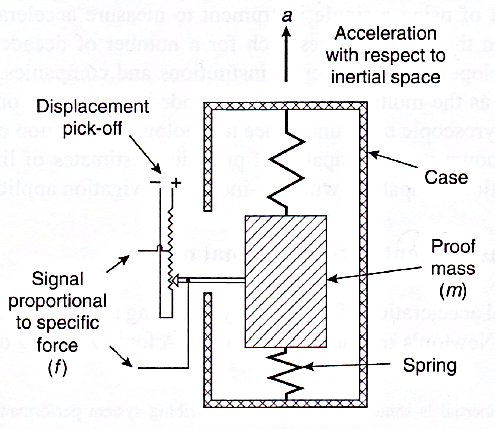
\includegraphics[scale=0.5]{figures/bProblemloesning/accelerometer_basic.png}
	\caption{På figuren ses opbygningen af et accelerometer med en indre masse, fjedre og den ydre kapsel. Det ses på den indre masse, at denne er forskubbet mod bunden af kapslen, grundet en acceleration af accelerometeret. \citep{TittertonWeston2004} (Modificeret)}
	\label{acc_simpelt}
\end{figure}\vspace{-.2cm}
Ethvert stillestående objekt påvirkes af +1 g i den positive, vertikale akse \citep{Serway2010}. Derfor vil et stillestående accelerometer altid påvirkes af $\pm$1g på én bestemt akse afhængig af sensorens orientering. Eksempelvis, hvis accelerometeret er placeret på et bord med dets positive y-akse i vertikal retning, da vil y-aksen blive påvirket med $+$1 g. I dette tilfælde vil de andre akser, henholdsvis x-, og z-aksen, ikke blive påvirket af nogen kræfter med antagelse om idelle betingelser. 

Accelerometre benyttes enten i en åben eller lukket kreds. I en åben kreds fastholdes den indre masse til et nulpunkt ved at være udspændt mellem to fjedre. Ved acceleration af den ydre kapsel bevæges den indre masse væk fra nulpunktet, hvorved ændringen for et single-akse accelerometer vil være proportional med kræften, som påvirker systemet. \newline
I en lukket kreds fastholdes den indre masse til et nulpunkt ved hjælp af magnetiske kræfter. Oftest påmonteres en spole på den indre masse, hvormed magnetfeltet forstærkes. Det er muligt at foretage mere præcise målinger omkring nulpunktet end ved ændringerne. Accelerometre med den lukkede kreds er derfor mere præcis end accelerometre med en åben kreds. \citep{TittertonWeston2004,Academic2016d,Serway2010}
